%\subsubsection{(TODO) The Carnot Engine, Revisited}
%Before moving onto the statistical definition of entropy, let's answer a question about Carnot engines that might have arose as we learned about entropy; 
%\textit{How can Carnot Engines run reversibly if macroscopic processes are not truly reversible?}The answer is twofold. First, as we mentioned before the Carnot process is an idealization. It involves two isothermal steps, and as we've discussed no process is truly isothermal, unless it ran for an infinitely long time. Second, you need to be careful what system your considering when you say a process is reversible. The heat engine has zero change in entropy. However, when it interacts with its surroundings it inevitably changes the surrounding's entropy as well. Actually modelling this change in entropy would be fiendishly difficult \textbf{Rio Help I'm not sure this is right}, but we'd expect a high level of idealization to be necessary to actually make it zero, and otherwise for it to be positive. We could try to get around this problem by isolating the engine, but the efficiency of the engine is less than 100\%, so it needs a source of energy outside the system.

\subsubsection{(Optional) The Carnot Efficiency, Revisited}
To finish off this section, I want to show you a neat proof of Carnot's theorem; This theorem tells us that the maximum efficiency of a heat engine is given by $\eta = 1- \frac{T_C}{T_H}$ (the efficiency of the Carnot engine), where $T_C$ is the coldest temperature within the cycle, and $T_H$ is the hottest temperature within the cycle. We will explore in this section how this follows from the second law of thermodynamics. This section is completely optional, and just for your curiosity\footnote{Like seriously, this is completely out of the scope of Science One}, though you have all the tools you need to prove it yourself. To review how a heat engine fundamentally works, it takes in some heat $Q_H$ from a hot reservoir at temperature $T_H$, does some work $W$ with that energy, and then throws away waste heat $Q_C$ into a cold reservoir at temperature $T_C$, before returning to its initial state. This is pictured below:
\begin{center}
    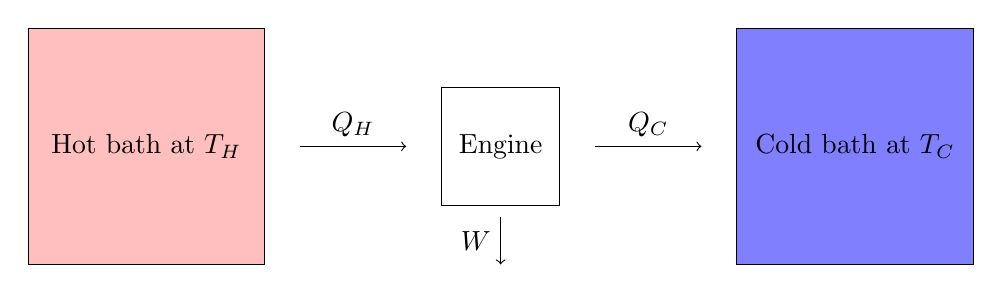
\begin{tikzpicture}[scale=3]
    \filldraw[fill=pink] (0,0) rectangle (1,1);
    \draw (1.75,0.25) rectangle (2.25,0.75);
    \filldraw[fill=blue!50] (3,0) rectangle (4,1);
    \draw[->] (1.15,0.5) -- (1.6,0.5);
    \draw[->] (2.4,0.5) -- (2.85,0.5);
    \draw[->] (2,0.2) -- (2,0);
    \node[above] at (1.375,0.5) {$Q_H$};
    \node[above] at (2.625,0.5) {$Q_C$};
    \node[left] at (2,0.1) {$W$};
    \draw (2,0.5) node {Engine};
    \draw (0.5,0.5) node {Hot bath at $T_H$};
    \draw (3.5,0.5) node {Cold bath at $T_C$};=
    \end{tikzpicture}
\end{center}


Now, let's consider the entropy of the hot reservoir, the engine, and the cold reservoir at the end of one cycle (in other words, we consider the change in entropy of the universe after one cycle). We recall that entropy is a function of state, and therefore at the end of a single cycle, the entropy of the heat engine itself must be the same as when it started. That is, $\Delta S_{engine} = 0$ for one full cycle. By the second law of thermodynamics $dS \geq \frac{Q}{T}$, the entropy of the hot reservoir decreases by the amount of heat $Q_H$ divided by its temperature $T_H$, so the entropy of the hot reservoir decreases by $\Delta S_{hot} \geq \frac{-Q_H}{T_H}$. Conversely, the cold reservoir increases in one cycle by $\Delta S_{cold} \geq \frac{Q_C}{T_C}$ (as it receives $Q_C$ heat at temperature $T_C$. Putting these together, we obtain the change in entropy of the universe for a single cycle:
\[\Delta S_{universe} \geq \frac{Q_C}{T_C} - \frac{Q_H}{T_H} \]
Now, the second law of thermodynamics tells us that the entropy of the universe must increase (or, to phrase it another way, if we treat the two reservoirs and the heat engine as an isolated system, the entropy of the total system must increase. This allows us to conclude that:
\[\Delta S_{universe} \geq \frac{Q_C}{T_C} - \frac{Q_H}{T_H} \geq 0 \]
So we obtain the important inequality:
\[\frac{Q_C}{T_C} - \frac{Q_H}{T_H} \geq 0 \]
Which we can rearrange to obtain:
\begin{equation}
    \label{eqn:(37)}
    \frac{T_H}{T_C} \geq \frac{Q_C}{Q_H}
\end{equation}
Note that to derive inequality \ref{eqn:(37)}, I have made no assumptions whatsoever about what my heat engine actually looks like; this is a completely general statement, based on the amounts of heat gained/lost from the hot/cold reservoirs, and the maximum/minimum hot/cold reservoir temperatures. Now, let us consider out definition of efficiency:
\begin{equation}
    \label{eqn:(38)}
    \eta = \frac{W}{Q_H}
\end{equation}
Where $W$ is the work done by the engine (what we get out), and $Q_H$ is the heat that we inject into the engine in one cycle from the hot reservoir (what we put in). By energy conservation, we find that:
\begin{equation}
    \label{eqn:(39)}
    W = Q_H-Q_C
\end{equation}
This might look like it came out of nowhere, so let's think about it a bit further. Just like entropy, internal energy is also a function of state; the energy something has doesn't care about how that energy got there! With this consideration, since the heat engine returns to the original state at the end of one cycle, just like the entropy change of the heat engine is zero in a single cycle, so must be the total internal energy; in other words, the heat engine must have the same energy it began with. With this consideration, we realize that the sum of the work done on the system and the heat given to the system must be 0, leading to equation \ref{eqn:(39)} above (work this out using the first law of thermodynamics if it's still unclear!). Now, we can substitute equation \ref{eqn:(39)} into equation \ref{eqn:(38)}, giving us:
\begin{align*}
    \eta = \frac{Q_H-Q_C}{Q_H} = 1 - \frac{Q_C}{Q_H}
\end{align*}
And now applying inequality \ref{eqn:(37)}, we have:
\begin{align*}
    1 - \frac{Q_C}{Q_H} \leq 1 - \frac{T_H}{T_C}
\end{align*}
And therefore:
\begin{equation}
    \eta \leq 1 - \frac{T_H}{T_C}
\end{equation}
We have hence proven Carnot's theorem, and can see that for any arbitrary heat engine, the efficiency is bounded by the Carnot efficiency. 
